\chapter{Physics Objects\label{ch:objects}}

After data is selected by the trigger, the offline analyses begin with particle identification.
There are no longer any timing limitations, so such identifications can make use of all the detector
information in the event. CMS uses the Particle Flow (PF) algorithm in most analyses, which is
described in Section~\ref{sec:PF}.
As this search centers around the identification of events with both $\Hgg$ and $\Hbb$ decays, the
identification and reconstruction of photons and jets are the first steps taken after the
trigger selects potentially-interesting events,
and this chapter discusses the treatments needed at this stage for both data and MC samples.
Recalling that the sensitivity in the separation between signal and background comes from the
excellend diphoton mass resolution, the identification of two high quality photons is the starting point
and discussed in Section~\ref{sec:photons}. The following step is the identification of two jets
coming from the hadronization of b-quarks and is discussed in Section~\ref{sec:jets}.


\section{Particle Flow\label{sec:PF}}

The PF algorithm recontructs all stable particles in an event from the digitized electronic signals
of all channels in all subsystems~\cite{PFPAS2009,CMS-PAS-PFT-10-001}. These particles include
electrons, photons, charged hadrons, neutron hadrons, and muons, as shown in Figure~\ref{fig:PF}.
From these particles, derived objects are constructed, including jets and missing transverse energy.
The algorithm itself links detector objects created from individual subsystems and groups them into
blocks that are identified with a particle. The detector objects are discussed in
Section~\ref{subsec:detobj}, the linking of these objects is discussed in Section~\ref{subsec:linking},
and the identification of groups of these links with particles is discussed in
Section~\ref{subsec:groupid}.

\begin{figure}[ht]
 \begin{center}
    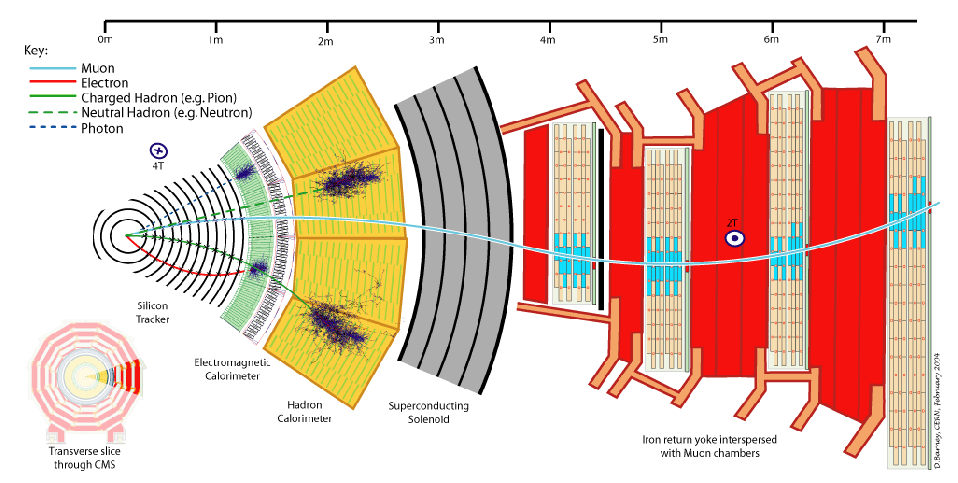
\includegraphics[width=0.95\textwidth]{figures/objects/pf.pdf}
      \end{center}
\caption{A schematic of a slice of the CMS detector in the plane transverse to the beam line.
The trajectories of an electron, photon, charged hadron, neutral hadron, and muon are superimposed
with the interactions that each of these particles would have with the various subsystems.}
\label{fig:PF}
\end{figure}

\subsection{Detector Objects\label{subsec:detobj}}

The first step of the PF algorithm is to assemble detector objects created separately from
individual subsystems. In the tracker, hits in pixels or strips are associated into a track candidate
through the iterative Combinatorial Track Finder algorithm~\cite{PFPAS2009}. In the muon chambers,
standalone muon tracks (to distiguish from tracks formed by tracker hits)
are assembled from hits in the three muon detectors, accounting
for the nonuniform magnetic field and large detector budget and contraining a track candidate to
intersect the beamline. In the ECAL and HCAL, clustering of energy deposits is performed around a
cluster seed, which is identified as a detector unit with an amount of energy exceeding a
detector-dependent threshold and corresponding to a local maximum.
Units are added to adjacent seeds if their energy exceeds a noise threshold, and the PF clusters are
formed by redistributing the the energy back to the cluster seeds, recalculating the position as a
weighted average over the energy of each contributing cluster.

\subsection{Linking\label{subsec:linking}}

The next step of the PF algorithm is to link the detector objects to assemble PF candidates.
Possible links are between a track and standalone muon track, between a tracker track and a cluster, and
between two clusters, each having their own associated linking parameters. A link is formed between
a track and standalone muon track when the two can be merged into a global track with a fit
having $\chi^2$ below a threshold. A link is formed between a track and a cluster when the extrapolation of the track is within a certain distance of the cluster position. A link is formed between two clusters
(either both in ECAL, both in HCAL, or one in each) when the two clusters are within a certain distance.

\subsection{Grouping and Identification\label{subsec:groupid}}

An ensemble of links creates a block, and identification proceeds interatively through PF candidates.
First, muons are identified from those blocks that contain a global track having a momentum
sufficiently close to the momentum of the contained track. Then electrons are identified from blocks
containing a track and an ECAL cluster where the track and energy cluster satisfy requirements
consistent with the signature of an electron. Next photons and hadrons are identified from blocks
containing a track and a cluster from either ECAL or HCAL. If the calibrated energy in the clusters is
greater than the sum of the momentrum of the associated tracks, PF photons or PF neutrons are created
from the difference. If the difference is less than the energy in the ECAL clusters, a PF photon is
created from the block; if the difference is greater than the energy in the ECAL clusters,
a PF photon and a PF neutral hadron are made from the excesses ECAL and HCAL energy, respectively.
Finally, if the calibrated energy in the clusters is less than the sum of the momentrum of the associated
tracks, a search for fake tracks and additional muons in the block is performed, and what remains
in the block is a PF charged hadron.

From the list of PF candidates in an event, jets and taus are constructed by clustering nearby
hadrons. In this way, the clustering of PF hadrons represents the original quark or tau from the
underlying interaction. Missing transverse energy, which is a signature of one or more neutrinos
in the event and/or the mismeasurement of the energy of PF candidate, is obtained by
\begin{equation}
\met = - \sum_i \vec{p}_{{\rm T},i} \, ,
\end{equation}
where the sum is over all PF candidates in the event.

The treatment for photons is discussed in more detail in Section~\ref{sec:photons}. The construction
of jets from PF candidates is discussed in more detail in Section~\ref{sec:jets}. 


%Matching the muons to the tracks measured in the silicon tracker results in a transverse momentum
%resolution between 1 and 5\,\% for \pt values up to 1~TeV. The ECAL has an energy resolution better
%than 0.5\% for unconverted photons with transverse energies above 100~GeV.
%The HCAL, when combined with the ECAL, measures jets with a resolution
%$\Delta E/E \approx 100\,\% / \sqrt{E\,[\gev]} \oplus 5\,\%$.

\section{Photons\label{sec:photons}}

Resume here!!!

Photon candidates are reconstructed from clusters of energy in the ECAL using the default
CMS algorithms [23].  In order to obtain the best energy resolution the calorimeter signals are
calibrated and corrected for several detector effects [24].   A multi-step procedure is used to
correct the energy scale in data and to determine Gaussian smearings which are applied to
the simulated photons to reproduce the same energy resolution in simulation as observed in
data.

Once the photon candidates are built, a selection to identify isolated photons is applied to
separate prompt photons from objects reconstructed as a photon which come from jets or from
misidentified electrons.  This selection consists of an electron veto, a selection on the hadronic
leakage of the shower and some requirements based on the electromagnetic shower shape and
on isolation variables.

The two photons are requested to satisfy the asymmetric cut
p
T
,
g
1
/
m
gg
>
1/3 and
p
T
,
g
2
/
m
gg
>
1/4, where
p
T
,
g
1
and
p
T
,
g
2
are the transverse momenta of the leading and sub-leading photons.
The use of transverse momentum thresholds scaled by the diphoton invariant mass prevents
turn-on effects which may distort the shape of the low mass end of the
m
gg
spectrum.  Both
photons are required to be within the ECAL acceptance
j
h
g
j
<
2.5 and the transition region
between the ECAL barrel and the ECAL endcaps is excluded.  If more than two photons are
reconstructed which pass the above requirements, the two with highest transverse momentum
are selected for the analysis.  A pre-selection 100
<
m
gg
<
180 GeV is applied.  The resulting
simulated signal mass shape of the Higgs decaying into two photons is shown on the Figure 1
(top-left), and compared to the sum of all standard model production mechanisms of a single
Higgs decaying to two photons.  The trigger efficiency for the above-mentionned selection is
measured to be larger than 99%.
The typical resolution in the diphoton mass spectrum for the signal is 1 GeV. It is driven by
the photon energy resolution and the knowledge about the direction of the photons, which is
in turn dominated by the knowledge of the vertex from which they originate.  The presence
of a second Higgs decaying to jets allows us to efficiently identify the event vertex as the one
with the largest value of
Â
p
2
T
, where the sum runs over all the tracks associated to the vertex.
The relative contribution from the vertex assignment to the diphoton mass resolution becomes
negligible with respect to the photon energy resolution when the distance between the chosen
vertex and the true one is below 1 cm. Considering this tolerance the vertex finding efficiency
exceeds 99 %.

\section{Jets\label{sec:jets}}



